\chapter{Ordinary Differential Equations}
\begin{defn}
  A \textbf{differential equation} is an equation involving derivatives.
\end{defn}
\begin{defn}
  A \textbf{direction field} tells us the slope of a function at any given place.
\end{defn}
\begin{ex}
    In physics, we often define acceleration to be a vector relative to another 
    vector, velocity.
    Here, we will just consider them as scalars for the sake of argument.
    Acceleration is a change in velocity, so
    \begin{equation}
        a = \leib{v}{t},
        \label{eq:acceleration}
    \end{equation}
    where $v$ represents velocity and $t$ represents time.
    Now we integrate both sides of \eref{eq:acceleration} with respect to $t$,
    \begin{equation}
        \int a \ud t = \int \leib{v}{t} \ud t.
        \label{eq:intaccel}
    \end{equation}
    Now, assuming\footnote{This must be explained later, but as a warning: no,
    the $\ud t$ in the derivative operation and the $\ud t$ in the integration 
    operation do not simply cancel.}
    \begin{equation}
        \int \leib{v}{t} \ud t = \int \ud v,
        \label{eq:handwave}
    \end{equation}
    then using \eref{eq:handwave}, we see that
    \begin{equation}
        \int a \ud t = \int \ud v.
        \label{eq:naughtint}
    \end{equation}
    From here we simplify, finding that
    \begin{equation}
        at + c_1 = v + c_2.
        \label{eq:almostvelocity}
    \end{equation}
    The constants in \eref{eq:almostvelocity} are simply constants and may be combined into another constant, $C$.
    Also, the equation may be rearranged to put it in more familiar form, yielding
    \begin{equation}
        v = at + C,
        \label{eq:velocity}
    \end{equation}
    which we recognize as the classical mechanics equation for velocity.
    Integrating once more, and replacing $v$ with the definition of velocity as change in position, we find
    \begin{align}
        \int \leib{x}{t} \ud t &= \int (at + C) \ud t, \nonumber \\
        \int \leib{x}{t} \ud t &= \int at \ud t + \int C \ud t, \nonumber \\
        x + c_3  &= a \frac{t^2}{2} + Ct + c_4. \nonumber \\
        \intertext{Now we may simply combine the constants once more, defining $C_1$ to constitute the difference of $c_4$, and $c_3$,}
        x &= a \frac{t^2}{2} + Ct + C_1. \label{eq:phys_const}
    \end{align}
    \eref{eq:phys_const} may be rewritten in its more common form:
    \begin{equation}
        x(t) = \frac{1}{2} a t^2 + v_0 t + x_0.
        \label{eq:position}
    \end{equation}
\end{ex}

\section{Second-order differential equations with linear combination solutions}

\section{Linear, homogeneous}

\[ ay'' + by'' +cy = 0 \]

Each coefficient is a constant. We come up with a 
characteristic equation\index{characteristic equation}

\[ ar^2 +br + c = 0 \]

Which is quadratic.

\begin{enumerate}
    \item We get two distinct solutions, meaning $r1 \neq r2$. this implies 
        $r1, r2 \in \mathbb{R}$ and our characteristic equation is of the form
        $y = c_1 e^{r_1t}+c_2e^{r_2t}$.
    \item $r1 = r2 $, and $r1, r2 \in \mathbb{C}$,
        meaning we still have a general solution of the form
        $y = c_1 e^{r_1t} + c_2 e^{r_2t}$, where $r_1,\quad r_2$ are of the form
        $\alpha \pm \beta i$. Note that our general solution here is in what
        is called ``linear combination form,'' and we will change this later.
    \item $r_1=r_2=r$, where $r \in \mathbb{R}$.
        This implies a general solution of the form $y=c_1e^{rt}+c_2te^{rt}$.
\end{enumerate}

\begin{ex}
    \begin{equation}
        y'' + 4y' + 4y = 0
        \label{eq:sec_ord_ode}
    \end{equation}
    \begin{enumerate}
        \item[(a)] Find one solution, $y_1 (t)$.
        \item[(b)] Show that $y_2(t) = ty_1(t)$ is also a solution.
        \item[(c)] Give the general solution.
    \end{enumerate}
    \begin{sol}
        \begin{enumerate}
            \item[(a)] Characteristic equation:
                \begin{align} 
                    r^2 + 4r + 4 &= 0 \\
                    (r + 2) ^2   &= 0
                \end{align}
                This implies that $r = - 2$, and therefore $y_1(t)= e^{-2t}$
                is a solution to \eref{eq:sec_ord_ode}.
            \item[(b)]
                \begin{align}
                    y_2    (t) &= t e^{-2t} \\
                    y_2 '  (t) &= e^{-2t} - 2 t e^{-2t} \\
                    y_2 '' (t) &= -2 e^{-2t} - 2 e^{-2t} + 4t e^{-2t} \\
                \end{align}
                To test this, we show that
                \[ -2e^{-2t} - 2e^{-2t} + 4te^{-2t} + 4e^{-2t} -8te^{-2t} + 4te^{-2t} = 0, \]
                which it does, so our solution is correct.
            \item[(c)]
                The general solution will be a linear combination of $y_1$
                and $y_2$:
                \[ y = c_1 e^{-2t} + c_2te^{-2t}. \]
        \end{enumerate}
    \end{sol}
\end{ex}

\section{Principle of Superposition}
If $y_1, y_2$ are solutions to $L(y) = y'' +g(t) y' + r(t) y = 0$, then
$y=c_1 y_1 + c_2 y_2$ is a solution to $L(y) = 0$.

The proof for this is found by plugging $y''$ and $y'$ into $L(y)$, and showing
that the result equals zero.

\begin{theorem}
    If $y_1, y_2$ are solutions to $L(y) = 0$, then $y=c_1y_1 + c_2 y_2$ is the
    general solution, iff:

    \begin{equation}
        \wronk{y_1, y_2} = 
        \begin{vmatrix}
            y_1(t)  & y_2(t) \\
            y_1'(t) & y_2'(t)
        \end{vmatrix}
        \neq 0
    \end{equation}
\end{theorem}

\begin{ex}
    If $y_1=t$ and $\wronk{y_1, y_2} = t^2 e^t$, find $y_2(t)$.
    \begin{sol}
        \begin{align*}
            y_1(t) y_2 ' (t) - y_2 (t) y_1'(t) &= t^2 e^t \\
            y_1(t)\lieb{y_2 (t)}{t} - y_2(t) \leib{y_1(t)}{t} &= t^2 e^t \\
            t \leib{y_2(t)}{t} - y_2(t) &= t^2 e^t \\
            \leib {y_2}{t} - \frac{y_2(t)}{t} &= t e^t
        \end{align*}
        Let $\mu (t) = e^{\ln t} = - 1/t$ and we find that
        \[ \frac{y_2(t)}{t} = e^t + C. \]
    \end{sol}
\end{ex}
\section{Second-order linear homogeneous differential equations with constant coefficients}
A \textbf{second-order linear homogeneous} differential equation with 
\textbf{constant coefficients} is of the form
\begin{equation}
    a y'' + by' + cy = 0.
\end{equation}
\begin{ex}
    Solve the initial value problem
    \begin{equation}
        y'' + 4y' +5y = 0,
        \label{eq:2013-nov-ivp}
    \end{equation}
    where $y(0) = 1$ and $y'(0) = 0$.
    \begin{sol}
        From \eref{eq:2013-nov-ivp} we have the characteristic equation
        \begin{equation}
            r^2 +4r +5 = 0,
            \label{eq:2013-nov-ivp-char}
        \end{equation}
        which implies that
        \begin{align*}
            r_{1,2} &= \frac{
                -4 \pm \sqrt{4^2 - 4 \times 5}
            }{
                2
            } \\
            r_{1,2} &= \frac {
                -4 \pm \sqrt{4-5}
            }{
                2
            }\\
            r_{1,2} &= -2 \pm \sqrt{-1} \\
            r_{1,2} &= -2 \pm \iu
        \end{align*} 
        Thus
        \[ y_{1,2} = \ec ^ {(-2 \pm \iu ) t} \]
        are solutions to \eref{eq:2013-nov-ivp}.
    \end{sol}
\end{ex}
\section{Euler's identity}
\begin{equation}
    \ec ^{it} = \cos t + \iu \sin t
\end{equation}
\begin{equation}
    \ec^{\pi \iu} = -1
\end{equation}
\begin{equation}
    \ec^{\pi \iu} + 1 = 0
    \label{eq:euler-identity}
\end{equation}
\begin{remark}
    The number $\ec$ is defined in the equation
    \begin{equation}
        \int^\ec_1 \frac{1}{t} \ud t
    \end{equation}
    \begin{figure}[H]
        \begin{center}
            \includegraphics[width=0.4\textwidth]{continuous/ode/defn_e}
            \caption{$\ec$ is the number that makes the shaded area equal to $1$.}
        \end{center}
    \end{figure}
\end{remark}
% \section{Integrating Factors}
% We will observe differential equations of the form
% \begin{equation}
%   \leib{y}{t} = g(t) y + r(t)
% \end{equation}
% \begin{enumerate}
%   \item $\leib{y}{t} = t^2 y + \cos{t}$
%   \item $t y +3=\leib{y}{t}-2t$
% \end{enumerate}
